\documentclass{article}
\usepackage{graphicx} % Required for inserting images

\renewcommand{\familydefault}{\rmdefault}
\begin{document}

\title{\huge\textbf{Project Proposal \\ ComfortSphere - A Smart Home System for Indoor Environment Optimization}}

\author{Juhi Joshi (316800), Amardeep Mishra (316652), Hardikkumar Savaliya (313904), Mohammad Sheikh (312538), 
Riya Mariya Varghese (316773), Chaudhary Hammad (313955) }


    

\maketitle
\section{Introduction}
{The field of IoT-enabled smart home systems has seen exponential growth, with applications ranging from simple remote controls to complex, automated home ecosystems. ComfortSphere proposes an advanced smart room ecosystem tailored for optimal indoor climate control, leveraging precise sensor data and automated adjustments to address the specific needs of health-conscious individuals and those with respiratory issues.\\

Use Case: ComfortSphere caters to users who require real-time monitoring of temperature and humidity levels, particularly in environments where fluctuating indoor conditions can adversely affect health. For example, people with asthma or COPD often need consistent humidity levels; ComfortSphere provides this by dynamically adjusting indoor climate factors in response to sensor readings and user preferences.\\

Broader Relevance: The relevance of automated climate control extends beyond individual well-being. It offers energy savings and security, impacting not only personal health but also the broader goals of sustainable energy consumption and indoor air quality improvement. By addressing this need, ComfortSphere is designed for a wide audience, from homeowners to healthcare and security engineers, with applications in residential and healthcare facilities.\\

Scope: The research focuses on integrating and optimizing smart sensors (DHT22, light, and motion sensors), microcontroller programming (using Pinecone), and app-based remote access to manage and monitor indoor climate parameters.
}

\section{Literature Review}
This section reviews the current research on smart home automation, sensor-based environmental monitoring, health impacts of indoor air quality (IAQ), and energy-efficient automation, assessing their contributions and limitations. By identifying gaps in the existing literature, ComfortSphere is positioned as an innovative solution that addresses the combined needs of health, energy savings, and convenience in indoor climate control.\\

1. Humidity-Based Temperature Control Using IoT
The research [1] “Humidity Based Automated Room Temperature Controller Using IoT” explores a humidity-based automated room temperature control system using IoT, implementing an electric heater for precise climate regulation. This system dynamically adjusts the fan speed based on temperature fluctuations, supported by an advanced sensor and controller setup. Unlike traditional analog systems, it leverages smart technology for more responsive temperature adjustments, allowing users to tailor indoor climate settings to their comfort and health needs. However, this system is mainly designed for temperature control without integration of user-specific health metrics or energy-efficient features, which ComfortSphere aims to address by including additional health-focused adjustments and motion-sensor integration for energy savings.\\

2. Air Quality Monitoring in Medical Settings
A study on air quality monitoring in hospital rooms by [2] “Air Quality Monitoring and Control System for a Hospital Room” emphasizes cost-effective solutions for continuous temperature and humidity monitoring, with an added Bluetooth module for remote control. The system aims to improve patient care by providing real-time data, making it suitable for resource-limited settings. While the system shows great potential for healthcare, it primarily targets hospitals and lacks customizable user settings specific to home environments. ComfortSphere builds upon this by offering a more versatile and user-centric solution that includes remote accessibility, allowing users to monitor and adjust IAQ through a mobile app, benefiting individuals with respiratory conditions at home.\\

3. Portable Humidity and Temperature Monitoring Nodes
The portable node described in [3] ”A portable node of humidity and temperature sensor for indoor environment monitoring” is a compact, cost-effective system designed for smart home monitoring, featuring a DHT11 sensor, Zigbee module, STM32L100 microcontroller, and a smartphone interface. Its portability and low-power consumption make it convenient for indoor monitoring. However, the system’s capabilities are limited to basic data collection and do not extend to automated climate adjustments or health-specific features. ComfortSphere advances this concept by integrating a DHT22 sensor with higher precision and incorporating motion-sensing for adaptive, energy-efficient automation, allowing it to serve not only as a monitoring tool but as a health-oriented, automated climate control system.\\

4. Intelligent Indoor Temperature and Humidity Control
The indoor climate control system designed in [4]“Intelligent Indoor Temperature and Humidity Control System” aims to overcome the limitations of traditional climate control by using wireless communication and control algorithms, adjusting settings to maintain ideal temperature and humidity levels. The use of wireless modules and real-time monitoring enables the system to control HVAC components like air conditioners and humidifiers, enhancing user comfort. While this system is effective in maintaining a stable indoor environment, it lacks real-time, health-specific calibrations and personalized climate adjustments. ComfortSphere fills this gap by dynamically optimizing IAQ based on user-defined health needs, offering personalized adjustments for individuals with asthma or COPD.\\

5. Intelligent Monitoring for Indoor Environments
In [5]“Indoor Environment Intelligent Monitoring System”, the development of an indoor environmental monitoring system leverages an STM32 microcontroller and SHT10 sensor to track the indoor temperature and humidity data. Users can remotely access real-time and historical data, enabling them to observe trends and system performance. Although long-term testing confirms the system’s stability and accuracy, it primarily functions as a monitoring solution without active climate control capabilities. ComfortSphere extends this approach by not only monitoring but actively adjusting indoor conditions to improve IAQ for health-conscious users, integrating motion-based automation for added energy efficiency.\\

6. Smart Light Using PIR Sensor
The study [7] “Smart Light Using PIR Sensor” aligns with the adaptive lighting goals of ComfortSphere by employing motion detection to conserve energy and enhance user convenience. It proposes efficient, scalable, and cost-effective lighting solutions that can be seamlessly integrated into broader smart home systems like ComfortSphere. Unlike standalone lighting systems, ComfortSphere combines PIR-based adaptive lighting with other health and energy-efficient features, offering a holistic approach to smart home automation.\\

7. Health Impacts of Humidity on Respiratory Well-Being
Research by [6] “Effects of Low Humidity and High Humidity on the Nasal Area of the People” investigates how varying humidity levels influence respiratory health, particularly through symptoms like nasal congestion, dryness, and sneezing. Findings show that exposure to low humidity can lead to nasal and skin dryness, while high humidity increases congestion. This study highlights the need for systems that maintain a balanced indoor climate, which is essential for individuals with respiratory sensitivities. ComfortSphere aligns with these findings by maintaining optimal humidity levels (40-60%) to prevent health issues associated with poor IAQ, based on WHO recommendations, making it a health-supportive alternative to standard smart thermostats.



By addressing limitations in each of these studies, ComfortSphere contributes to the evolving field of IoT-enabled smart home systems, focusing on adaptive climate control to promote respiratory health, user-centric customization, and energy-efficient automation.

\section{Research Questions}
The primary research question guiding this project is:\\

How effectively can ComfortSphere manage and optimize indoor environmental conditions to support health and energy efficiency in a smart home setting?\\

Sub-questions include:\\

How accurately does the DHT22 sensor maintain optimal temperature and humidity levels in real time?\\

What measurable impact does automated climate control, based on occupancy data, have on energy savings?\\

To what extent does the motion-sensor integration enhance safety and convenience in daily use?\\

How does the ComfortSphere app improve user engagement with indoor environment monitoring and adjustments?\\

\section{Methodological Design}
\begin{figure}
    \centering
    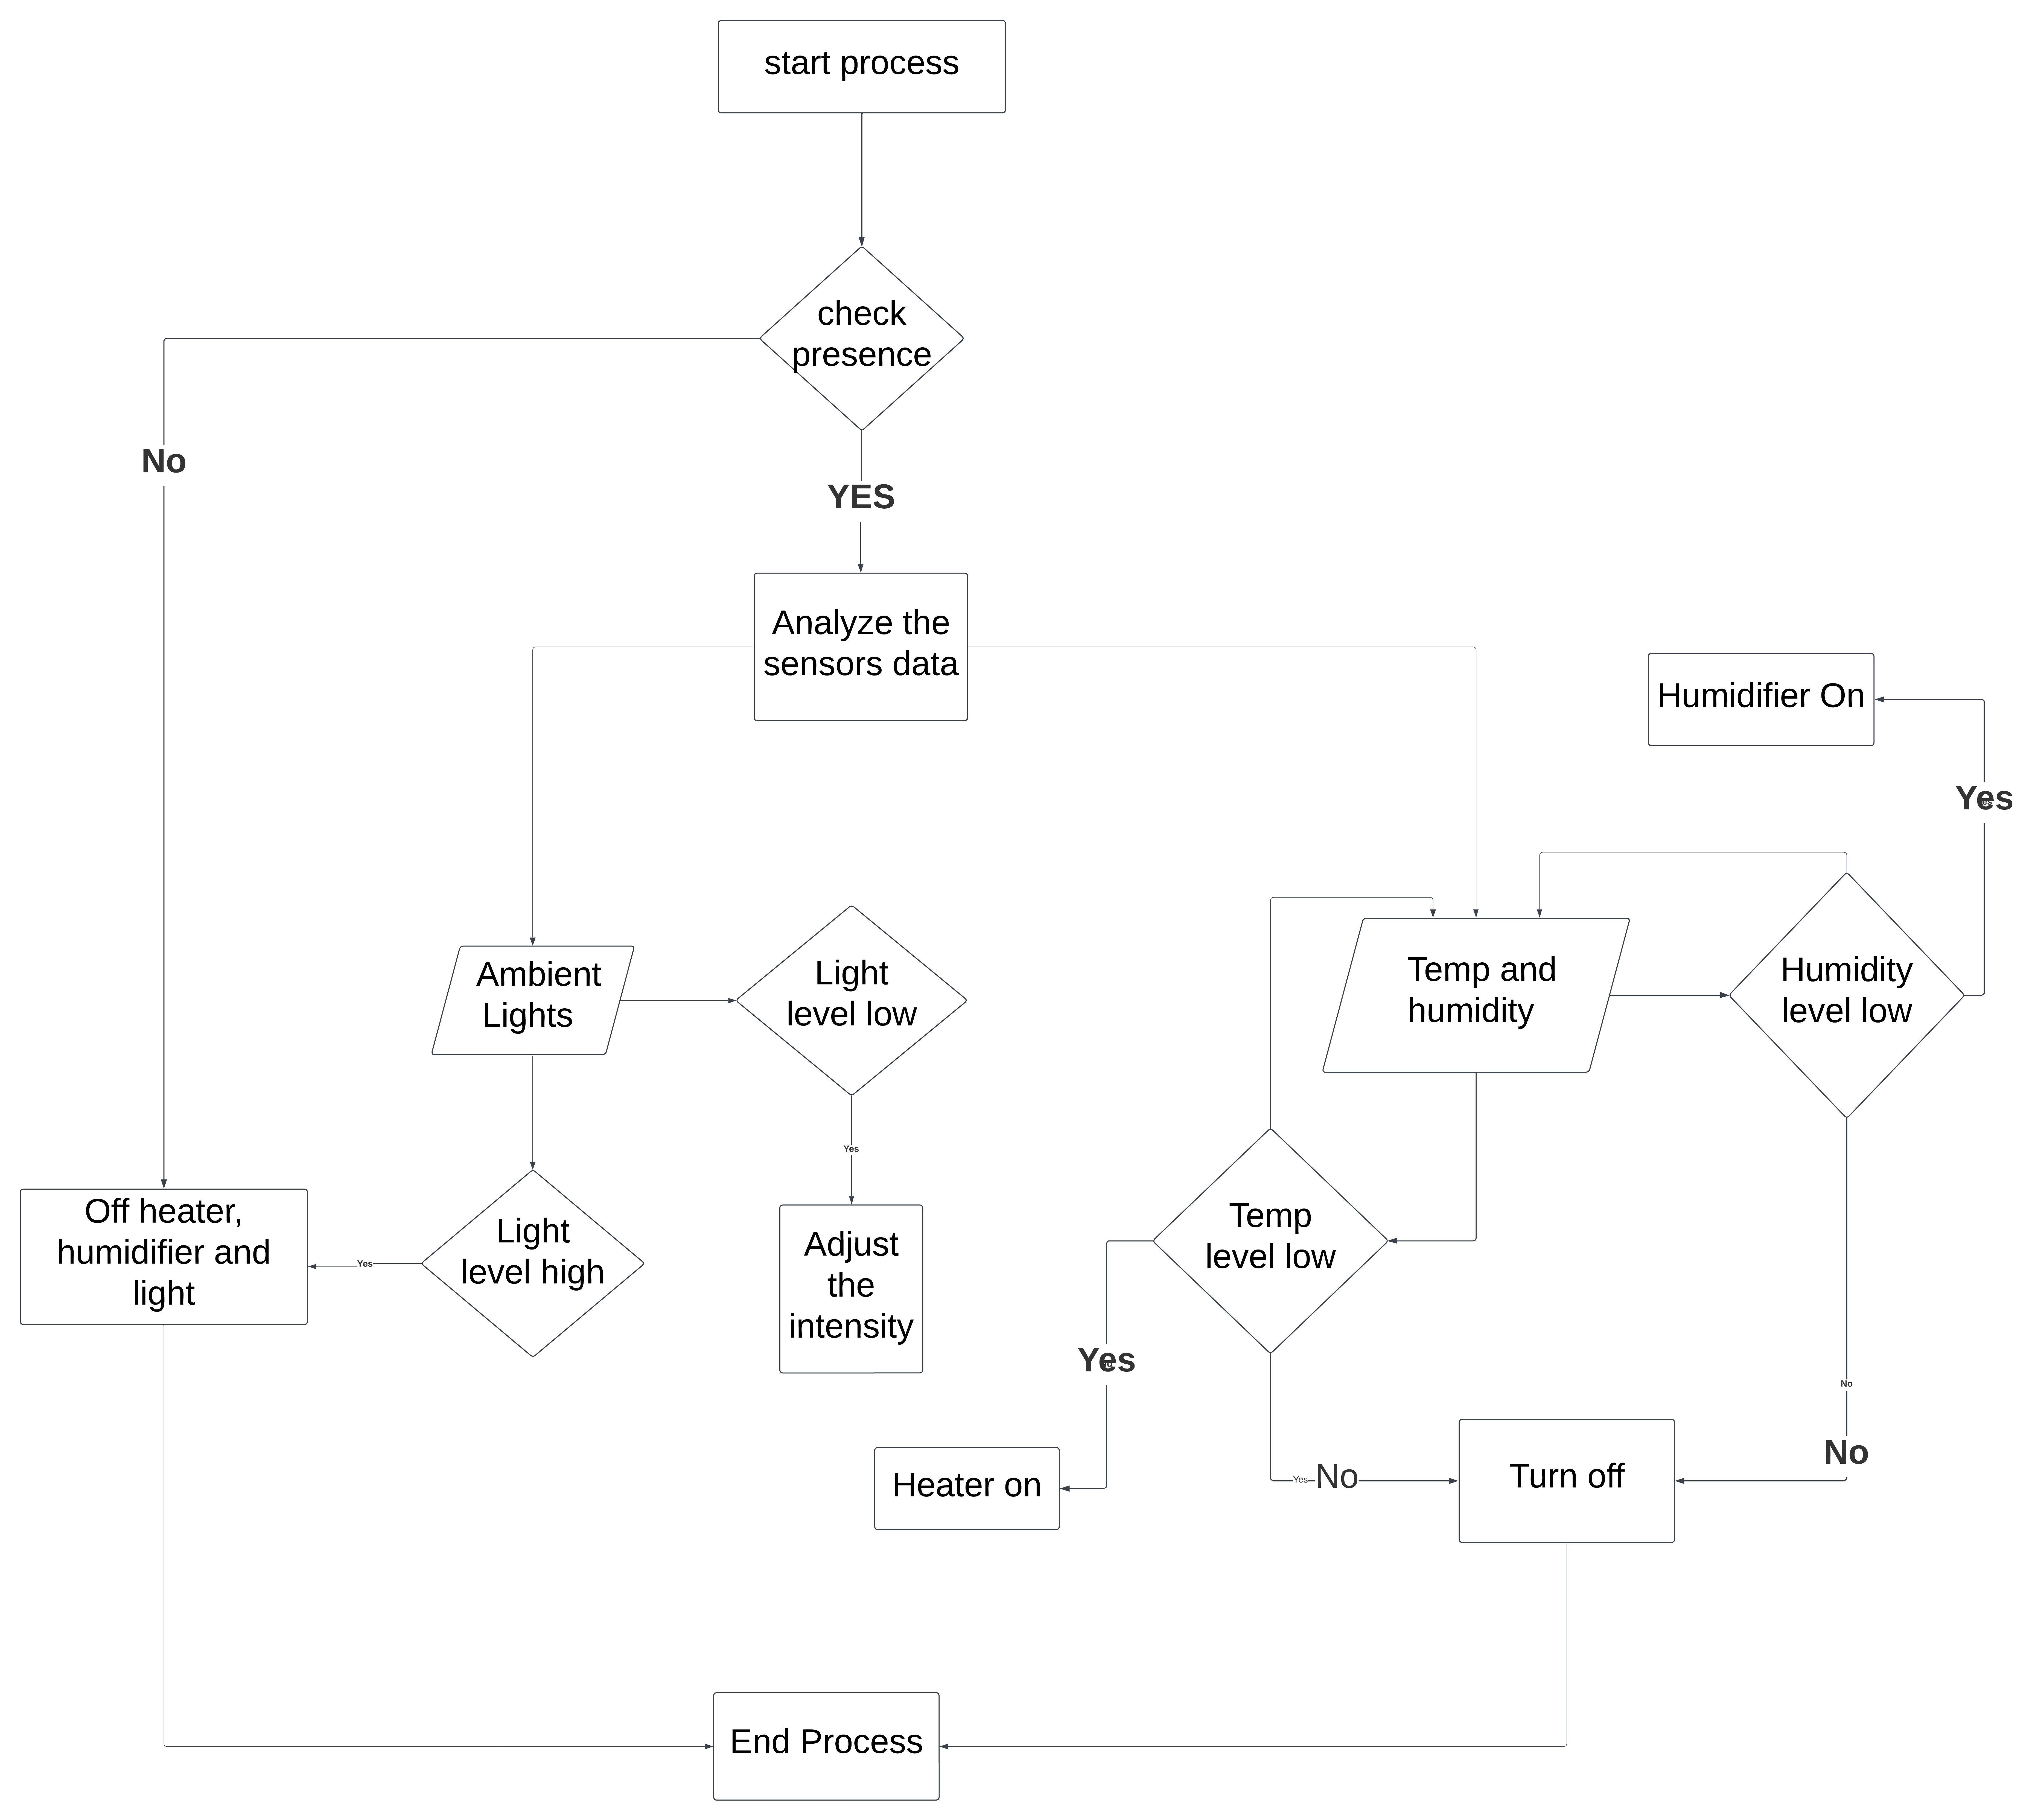
\includegraphics[width=0.5\linewidth]{diagram.jpg.png}
    \caption{Enter Caption}
    \label{fig:enter-label}
\end{figure}
The methodological design includes experimental setup, data processing, and user interaction with the ComfortSphere System.\\

\begin{enumerate}
    \item Approach
This study will employ a quantitative experimental approach, testing system accuracy, response time, and energy efficiency across various use cases. The qualitative component will involve user feedback on system usability and perceived health benefits.
    \item Data Collection and Access
\begin{itemize}
    \item Sensors: Data will be collected using the DHT22 (for temperature and humidity), an occupancy-detecting motion sensor. and a light sensor for ambient lightning. Sensor readings will be continuously logged via the Pinecone microcontroller, and then transmitted to the ComfortSphere app.
\end{itemize}
\begin{itemize}
    \item User Interaction: Users will interact with the app to set climate preferences, toggle lights, monitor real-time data, and review historical records. User feedback will be collected through surveys and structured interviews to assess satisfaction and health impacts.
\end{itemize}

    \item Use Cases and Experiment Selection

    Three specific user profiles will be included:
\begin{itemize}
    \item Health-focused: Users with asthma or respiratory concerns.

    \item Energy-conscious: Users prioritize cost and energy efficiency.
    \item Safety-conscious: Elderly or vulnerable individuals for whom safety features are vital.
\end{itemize}

    \item Each group will use the system for two weeks, after which data on system performance, energy use, and user 
satisfaction will be analyzed.
    \item Time Frame
The experimental phase will last approximately three months, including setup, data collection, and user feedback. An additional month will be allocated for data analysis, system calibration, and refinement.
    \item Data Recording and Processing
\begin{itemize}
    \item Data Recording: Sensor data will be recorded on the Pinecone microcontroller and transmitted to a cloud server, accessible through the ComfortSphere app.

    \item Data Analysis: Quantitative data on temperature, humidity, and energy consumption will be processed using statistical software to analyze trends, variance, and correlation with user preferences and occupancy.
    \item User Feedback: Survey responses will be analyzed using thematic coding to identify patterns in user satisfaction and health-related feedback.
\end{itemize}
    \item Presentation of Findings
Results will be presented in graphical form (line charts for time-series data, bar charts for user feedback), with statistical analyses showing the correlation between environmental parameters and user-reported health outcomes.
\end{enumerate}
\end{document}
